%-------------------------------------------------%
\subsection{Modelo: K-Nearest Neighbor (kNN)}
%-------------------------------------------------%
Vecinos mas cercanos:\\
Este algoritmo busca las ``k" observaciones mas parecidas del conjunto de entrenamiento al registro que se está evaluando que pertenece al conjunto de test. De esos k registros mas parecidos, se extrae la clase y cuyo valor sea el predominante, será el que se le otorgue al registro de Test.


%-------------------------------------------------%
\subsubsection{Determinar parámetros del modelo}
%-------------------------------------------------%
Éste método tiene un hiperparámentro solo (k), que hace referencia a la cantidad de registros vecinos que el algoritmo evaluará para luego clasificar según la clase predominante.\\

Para realizar el modelo se emplea validación cruzada con 10 particiones y 5 repeticiones. A su vez, cada iteración se repite con distintos valores del hiperparámetro k. En este caso se optaron por 6 valores: (1, 2, 5, 10, 15, 20, 30, 50, 60, 70, 80).\\
Entonces se puede decir que se realizan: 10*5*6 = 300 modelos, y de todos ellos se obtiene el mejor.

Las diferentes ejecuciones para elegir el parámetro óptimo se visualizan en la tabla \ref{tab:knn_corridas_parametros}.
Se puede determinar que el mejor resultado se obtiene con un k=70 y accuracy de 81,27\%.


\begin{table}[!h]
	
	\caption{\label{tab:knn_corridas_parametros} Ejecuciones de knn con diferentes parámetros}
	\centering
	\begin{tabular}[t]{rrrrr}
		\toprule
		\rowcolor{black}  \multicolumn{1}{c}{\textcolor{white}{\textbf{k}}} & \multicolumn{1}{c}{\textcolor{white}{\textbf{Accuracy}}} & \multicolumn{1}{c}{\textcolor{white}{\textbf{Kappa}}} & \multicolumn{1}{c}{\textcolor{white}{\textbf{AccuracySD}}} & \multicolumn{1}{c}{\textcolor{white}{\textbf{KappaSD}}}\\
		\midrule
		\rowcolor{gray!6}  1 & 0.7583 & 0.5077 & 0.0218 & 0.0451\\
		2 & 0.7535 & 0.4981 & 0.0216 & 0.0439\\
		\rowcolor{gray!6}  5 & 0.7956 & 0.5810 & 0.0202 & 0.0417\\
		10 & 0.7993 & 0.5877 & 0.0228 & 0.0477\\
		\rowcolor{gray!6}  15 & 0.8021 & 0.5937 & 0.0229 & 0.0476\\
		\addlinespace
		20 & 0.8033 & 0.5959 & 0.0204 & 0.0428\\
		\rowcolor{gray!6}  30 & 0.8049 & 0.5995 & 0.0209 & 0.0434\\
		50 & 0.8124 & 0.6144 & 0.0209 & 0.0437\\
		\rowcolor{gray!6}  60 & 0.8122 & 0.6140 & 0.0206 & 0.0430\\
		70 & 0.8127 & 0.6149 & 0.0209 & 0.0437\\
		\addlinespace
		\rowcolor{gray!6}  80 & 0.8096 & 0.6085 & 0.0224 & 0.0466\\
		\bottomrule
	\end{tabular}
\end{table}

\begin{figure}[!htb]
	\centering
	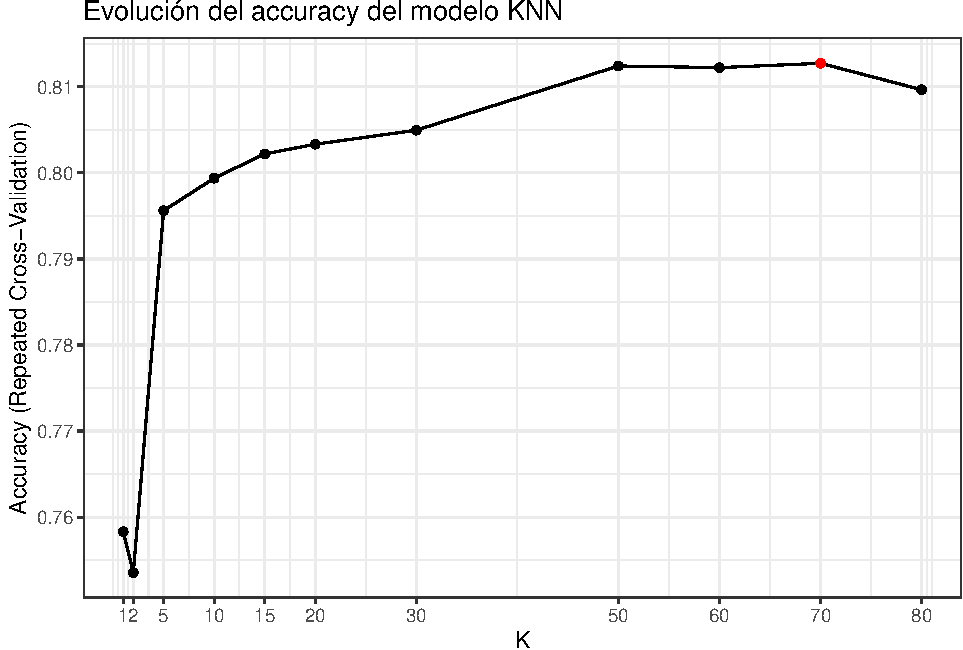
\includegraphics{imagenes/modelos_varios/unnamed-chunk-13-1.pdf}
	%\includegraphics[width=0.25\textwidth]{mesh}
	\caption{Evolución de Accuracy en modelos knn}
	\label{fig:knn_k_evolucion_accuracy}
\end{figure}


%-------------------------------------------------%
\subsubsection{Modelar}
%-------------------------------------------------%

Se ejecuta modelo de knn con k=70 utilizando todo el datset de train como entrenamiento (sin validación) obteniendo un accuracy de 81,98 \%, el cual es muy cercano al obtenido durante la búsqueda del parámetro óptimo (81,27\%)

%-------------------------------------------------%
\subsubsection{Describir el modelo}
%-------------------------------------------------%

Se evalúa el modelo anterior con el conjunto de Test cuyas observaciones no han sido utilizadas hasta ahora. Se detalla la Matriz de Confusión \ref{tab:MatrizConf_KNN} y algunas métricas \ref{tab:metricas_KNN}.

Como es de esperarse, los aciertos en el dataset de Test son menores que en el de entrenamiento. En este caso un 80.3 \% que sigue encontrándose muy por encima del nivel mínimo que corresponde a la
clase mayoritaria (56\%)



\begin{table}[!h]
	
	\caption{\label{tab:MatrizConf_KNN}Matriz de Confusión del método: KNN }
	\centering
	\begin{tabular}[t]{lcc}
		\toprule
		\multicolumn{1}{c}{Prediccion} & \multicolumn{1}{c}{Referencia} & \multicolumn{1}{c}{ } \\
		\cmidrule(l{3pt}r{3pt}){1-1} \cmidrule(l{3pt}r{3pt}){2-2}
		\rowcolor{black}  \multicolumn{1}{c}{\textcolor{white}{\textbf{ }}} & \multicolumn{1}{c}{\textcolor{white}{\textbf{0}}} & \multicolumn{1}{c}{\textcolor{white}{\textbf{1}}}\\
		\midrule
		\rowcolor{gray!6}  0 & 657 & 160\\
		1 & 110 & 440\\
		\bottomrule
	\end{tabular}
\end{table}

\begin{table}[!h]
	
	\caption{\label{tab:metricas_KNN}Métricas del metodo: KNN }
	\centering
	\begin{tabular}[t]{cc}
		\toprule
		\rowcolor{black}  \multicolumn{1}{c}{\textcolor{white}{\textbf{metricas}}} & \multicolumn{1}{c}{\textcolor{white}{\textbf{valor}}}\\
		\midrule
		\rowcolor{gray!6}  Accuracy & 0.8024\\
		Kappa & 0.5953\\
		\rowcolor{gray!6}  AccuracyLower & 0.7803\\
		AccuracyUpper & 0.8232\\
		\rowcolor{gray!6}  AccuracyNull & 0.5610\\
		\addlinespace
		AccuracyPValue & 0.0000\\
		\rowcolor{gray!6}  McnemarPValue & 0.0028\\
		Sensitivity & 0.7333\\
		\rowcolor{gray!6}  Specificity & 0.8565\\
		Pos Pred Value & 0.8000\\
		\addlinespace
		\rowcolor{gray!6}  Neg Pred Value & 0.8041\\
		Precision & 0.8000\\
		\rowcolor{gray!6}  Recall & 0.7333\\
		F1 & 0.7652\\
		\rowcolor{gray!6}  Prevalence & 0.4389\\
		\addlinespace
		Detection Rate & 0.3218\\
		\rowcolor{gray!6}  Detection Prevalence & 0.4023\\
		Balanced Accuracy & 0.7949\\
		\bottomrule
	\end{tabular}
\end{table}



%-------------------------------------------------%
\subsection{Modelo: Regresión Logística}
%-------------------------------------------------%

La Regresión logística permite estimar la probabilidad de una variable cualitativa binaria en
función de variables cuantitativas. Es un algoritmo que puede explicar
bien la respuesta en función de sus predictores. La relación como lo
dice su nombre es logarítmica, por lo que la relación entre las
probabilidades y las variables no es lineal. El incremento en 1 unidad de
una variable depende también del valor que tiene la variable en ese
momento (es decir, la posición en la curva logarítmica donde se
encuentra).

%-------------------------------------------------%
\subsubsection{Determinar parámetros del modelo}
%-------------------------------------------------%
No existen hiperparámetros. Como en este caso se utiliza el paquete glm,
hay que determinar que se realiza una regresión logística indicando
que el paquete utilice la familia binomial.


%-------------------------------------------------%
\subsubsection{Modelar}
%-------------------------------------------------%

Se ejecuta el modelo obteniendo durante el entrenamiento un Accuracy de 83.7\%.\\

No todas las variables son significativas, lo que
nos lleva a pensar que algunas variables están aportando la misma información.



%-------------------------------------------------%
\subsubsection{Describir el modelo}
%-------------------------------------------------%


Se evalúa el modelo entrenado con el conjunto de Test. En este caso, se
puede observar \ref{tab:MatrizConf_logistic} \ref{tab:metricas_logistic} que el modelo resulta ser bastante robusto obteniendo
casi el mismo valor en Accuracy que el modelo entrenado, 83,54\%. Es un
buen modelo para tener en cuenta y analizarlo mas en profundidad.

\begin{table}[!h]
	
	\caption{\label{tab:MatrizConf_logistic}Matriz de Confusión del metodo: Regresión Logística (todos los predictores) }
	\centering
	\begin{tabular}[t]{lcc}
		\toprule
		\multicolumn{1}{c}{Predicción} & \multicolumn{1}{c}{Referencia} & \multicolumn{1}{c}{ } \\
		\cmidrule(l{3pt}r{3pt}){1-1} \cmidrule(l{3pt}r{3pt}){2-2}
		\rowcolor{black}  \multicolumn{1}{c}{\textcolor{white}{\textbf{ }}} & \multicolumn{1}{c}{\textcolor{white}{\textbf{0}}} & \multicolumn{1}{c}{\textcolor{white}{\textbf{1}}}\\
		\midrule
		\rowcolor{gray!6}  0 & 702 & 160\\
		1 & 65 & 440\\
		\bottomrule
	\end{tabular}
\end{table}

\begin{table}[!h]
	
	\caption{\label{tab:metricas_logistic}Métricas del método: logistic }
	\centering
	\begin{tabular}[t]{cc}
		\toprule
		\rowcolor{black}  \multicolumn{1}{c}{\textcolor{white}{\textbf{metricas}}} & \multicolumn{1}{c}{\textcolor{white}{\textbf{valor}}}\\
		\midrule
		\rowcolor{gray!6}  Accuracy & 0.8354\\
		Kappa & 0.6599\\
		\rowcolor{gray!6}  AccuracyLower & 0.8146\\
		AccuracyUpper & 0.8546\\
		\rowcolor{gray!6}  AccuracyNull & 0.5610\\
		\addlinespace
		AccuracyPValue & 0.0000\\
		\rowcolor{gray!6}  McnemarPValue & 0.0000\\
		Sensitivity & 0.7333\\
		\rowcolor{gray!6}  Specificity & 0.9152\\
		Pos Pred Value & 0.8712\\
		\addlinespace
		\rowcolor{gray!6}  Neg Pred Value & 0.8143\\
		Precision & 0.8712\\
		\rowcolor{gray!6}  Recall & 0.7333\\
		F1 & 0.7963\\
		\rowcolor{gray!6}  Prevalence & 0.4389\\
		\addlinespace
		Detection Rate & 0.3218\\
		\rowcolor{gray!6}  Detection Prevalence & 0.3694\\
		Balanced Accuracy & 0.8242\\
		\bottomrule
	\end{tabular}
\end{table}




%-------------------------------------------------%
\subsection{Modelo: Analisis discriminante Lineal
	(LDA)}
%-------------------------------------------------%

Este algoritmo utiliza el teorema de Bayes, para estimar la probabilidad
de que una observación pertenezca a cada una de las clases de la
variable cualitativa según el valor de los predictores. Es un algoritmo
explicativo y puede discriminar mas de dos clases, aunque este no sea el
caso. En primer lugar, se calculan las probabilidades de
pertenencia de la observación a cada una de las clases y luego se asigna la clase cuya probabilidad resulta la mas alta.



%-------------------------------------------------%
\subsubsection{Determinar parámetros del modelo}
%-------------------------------------------------%

No tiene.


%-------------------------------------------------%
\subsubsection{Modelar}
%-------------------------------------------------%

Utilizando el conjunto de entrenamiento, se obtiene una métrica Accuracy del 82.6\%


%-------------------------------------------------%
\subsubsection{Describir el modelo}
%-------------------------------------------------%

Evaluando el modelo con el conjunto de Test, el modelo aparenta ser
bastante robusto obteniendo casi el mismo valor en Accuracy (82.26\%)
que en entrenamiento (82.6\%). \ref{tab:MatrizConf_LDA} \ref{tab:metricas_LDA}

\begin{table}[!h]
	
	\caption{\label{tab:MatrizConf_LDA}Matriz de Confusion del metodo: LDA }
	\centering
	\begin{tabular}[t]{lcc}
		\toprule
		\multicolumn{1}{c}{Prediccion} & \multicolumn{1}{c}{Referencia} & \multicolumn{1}{c}{ } \\
		\cmidrule(l{3pt}r{3pt}){1-1} \cmidrule(l{3pt}r{3pt}){2-2}
		\rowcolor{black}  \multicolumn{1}{c}{\textcolor{white}{\textbf{ }}} & \multicolumn{1}{c}{\textcolor{white}{\textbf{0}}} & \multicolumn{1}{c}{\textcolor{white}{\textbf{1}}}\\
		\midrule
		\rowcolor{gray!6}  0 & 704 & 174\\
		1 & 63 & 426\\
		\bottomrule
	\end{tabular}
\end{table}

\begin{table}[!h]
	
	\caption{\label{tab:metricas_LDA}Métricas del metodo: LDA }
	\centering
	\begin{tabular}[t]{cc}
		\toprule
		\rowcolor{black}  \multicolumn{1}{c}{\textcolor{white}{\textbf{metricas}}} & \multicolumn{1}{c}{\textcolor{white}{\textbf{valor}}}\\
		\midrule
		\rowcolor{gray!6}  Accuracy & 0.8266\\
		Kappa & 0.6407\\
		\rowcolor{gray!6}  AccuracyLower & 0.8054\\
		AccuracyUpper & 0.8463\\
		\rowcolor{gray!6}  AccuracyNull & 0.5610\\
		\addlinespace
		AccuracyPValue & 0.0000\\
		\rowcolor{gray!6}  McnemarPValue & 0.0000\\
		Sensitivity & 0.7100\\
		\rowcolor{gray!6}  Specificity & 0.9178\\
		Pos Pred Value & 0.8711\\
		\addlinespace
		\rowcolor{gray!6}  Neg Pred Value & 0.8018\\
		Precision & 0.8711\\
		\rowcolor{gray!6}  Recall & 0.7100\\
		F1 & 0.7823\\
		\rowcolor{gray!6}  Prevalence & 0.4389\\
		\addlinespace
		Detection Rate & 0.3116\\
		\rowcolor{gray!6}  Detection Prevalence & 0.3577\\
		Balanced Accuracy & 0.8139\\
		\bottomrule
	\end{tabular}
\end{table}



%-------------------------------------------------%
\subsection{Modelo: Árbol de Clasificación simple}
%-------------------------------------------------%

Se emplea el algoritmo de arboles de decisión C5.0. Los árboles son
fáciles de interpretar aun cuando las relaciones entre predictores son
complejas. Se pueden leer las ramas del árbol e interpretarlas como reglas para clasificar a cualquier observación.

%-------------------------------------------------%
\subsubsection{Determinar parámetros del modelo}
%-------------------------------------------------%

Si bien en estos algoritmos existen parámetros como cantidad de
observaciones en los nodos finales, máximo nivel de profundidad, etc. En este caso no se empleará ninguno dejando que el algoritmo determine cual es mejor corte en los mismos.

%-------------------------------------------------%
\subsubsection{Modelar}
%-------------------------------------------------%

Finalizado el entrenamiento, el Accuracy informado es del 85,52\%.

\begin{lstlisting}
## Decision tree:
## 
## ciclo_lectivo_de_cursada <= -0.1784513:
## :...Aprobado <= 2.816905: 1 (889/45)
## :   Aprobado > 2.816905: 0 (26/2)
## ciclo_lectivo_de_cursada > -0.1784513:
## :...Aprobado > 0.1499444: 0 (819/56)
##     Aprobado <= 0.1499444:
##     :...tipo_de_aprobacion_libre <= -0.1299698:
##         :...tipo_de_aprobacion_firmo <= -1.007704: 1 (64/26)
##         :   tipo_de_aprobacion_firmo > -1.007704: 0 (834/150)
##         tipo_de_aprobacion_libre > -0.1299698:
##         :...noAprobado > 0.6500659: 0 (56/17)
##             noAprobado <= 0.6500659:
##             :...Aprobado <= -0.5414899: 1 (281/94)
##                 Aprobado > -0.5414899:
##                 :...cant_recursada_regular_Recurso4vez > -0.2406067: 1 (40/12)
##                     cant_recursada_regular_Recurso4vez <= -0.2406067:
##                     :...tipo_de_aprobacion_libre > 1.48903: 1 (36/12)
##                         tipo_de_aprobacion_libre <= 1.48903:
##                         :...EsTecnico_SinDato <= 0: 0 (124/40)
##                             EsTecnico_SinDato > 0: 1 (22/8)
\end{lstlisting}

%-------------------------------------------------%
\subsubsection{Describir el modelo}
%-------------------------------------------------%

Evaluando el árbol con el conjunto de test, se obtiene un 83,24 \% de Accuracy. \ref{tab:MatrizConf_arbol} \ref{tab:metricas_arbol}

\begin{table}[!h]
	
	\caption{\label{tab:MatrizConf_arbol}Matriz de Confusión del método: árbol }
	\centering
	\begin{tabular}[t]{lcc}
		\toprule
		\multicolumn{1}{c}{Prediccion} & \multicolumn{1}{c}{Referencia} & \multicolumn{1}{c}{ } \\
		\cmidrule(l{3pt}r{3pt}){1-1} \cmidrule(l{3pt}r{3pt}){2-2}
		\rowcolor{black}  \multicolumn{1}{c}{\textcolor{white}{\textbf{ }}} & \multicolumn{1}{c}{\textcolor{white}{\textbf{0}}} & \multicolumn{1}{c}{\textcolor{white}{\textbf{1}}}\\
		\midrule
		\rowcolor{gray!6}  0 & 666 & 128\\
		1 & 101 & 472\\
		\bottomrule
	\end{tabular}
\end{table}

\begin{table}[!h]
	
	\caption{\label{tab:metricas_arbol}Métricas del método: arbol }
	\centering
	\begin{tabular}[t]{cc}
		\toprule
		\rowcolor{black}  \multicolumn{1}{c}{\textcolor{white}{\textbf{metricas}}} & \multicolumn{1}{c}{\textcolor{white}{\textbf{valor}}}\\
		\midrule
		\rowcolor{gray!6}  Accuracy & 0.8324\\
		Kappa & 0.6582\\
		\rowcolor{gray!6}  AccuracyLower & 0.8116\\
		AccuracyUpper & 0.8519\\
		\rowcolor{gray!6}  AccuracyNull & 0.5610\\
		\addlinespace
		AccuracyPValue & 0.0000\\
		\rowcolor{gray!6}  McnemarPValue & 0.0857\\
		Sensitivity & 0.7866\\
		\rowcolor{gray!6}  Specificity & 0.8683\\
		Pos Pred Value & 0.8237\\
		\addlinespace
		\rowcolor{gray!6}  Neg Pred Value & 0.8387\\
		Precision & 0.8237\\
		\rowcolor{gray!6}  Recall & 0.7866\\
		F1 & 0.8047\\
		\rowcolor{gray!6}  Prevalence & 0.4389\\
		\addlinespace
		Detection Rate & 0.3452\\
		\rowcolor{gray!6}  Detection Prevalence & 0.4191\\
		Balanced Accuracy & 0.8274\\
		\bottomrule
	\end{tabular}
\end{table}


%-------------------------------------------------%
\subsection{Modelo: Random Forest}
%-------------------------------------------------%

Este algoritmo combina el proceso de bagging (bootstrap aggregation
-muestras de observaciones con repetición-) con distintos modelos de
árboles que toman features al azar. Al final promedia los modelos y
consigue reducir la varianza.


%-------------------------------------------------%
\subsubsection{Determinar parámetros del modelo}
%-------------------------------------------------%

Se utiliza el paquete ranger en el cual se pueden definir los siguientes
hiperparámetros:

\begin{itemize}
	\item
	mtry: número predictores seleccionados aleatoriamente en cada árbol.
	Se eligen para evaluar los valores: 3, 4, 5, 7.
	\item
	min.node.size: tamaño mínimo que tiene que tener un nodo para poder
	ser dividido. Se eligen para evaluar los valores: 2, 3, 4, 5, 10, 15,
	20, 30.
	\item
	splitrule: criterio de división. El criterio elegido es ``gini''.
\end{itemize}

El mejor modelo determinado queda con los siguientes parámetros: mtry=5,
splitrule=gini y
 min.node.size=30 según la evolución del accuracy \ref{fig:rf_hiperparam}


\begin{figure}[!htb]
	\centering
	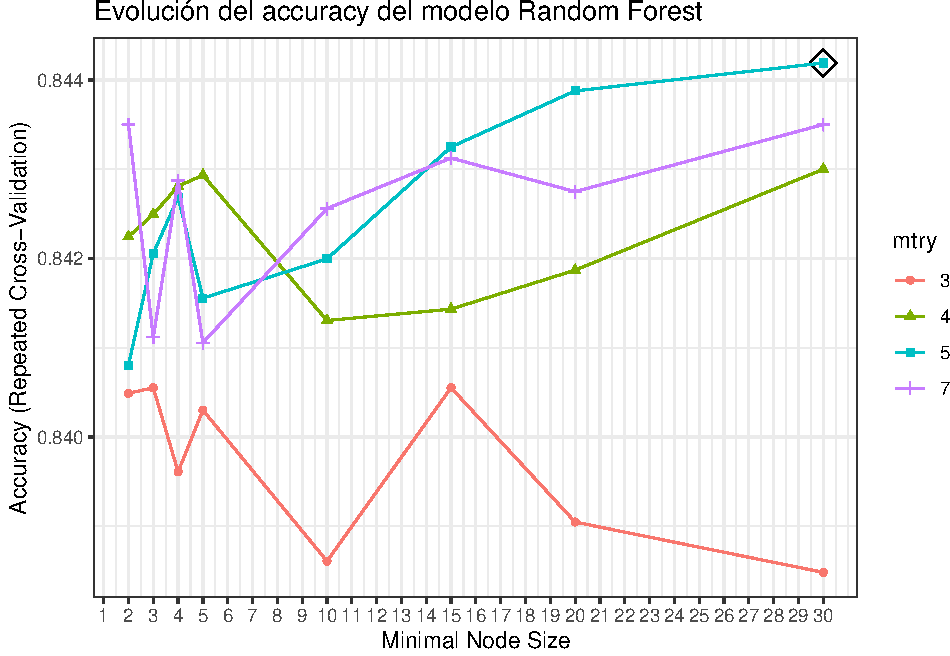
\includegraphics{imagenes/modelos_varios/unnamed-chunk-24-1.pdf}
	%\includegraphics[width=0.25\textwidth]{mesh}
	\caption{Evolución de Accuracy en modelos Random Forest para determinar hiperparámetros}
	\label{fig:rf_hiperparam}
\end{figure}



%-------------------------------------------------%
\subsubsection{Modelar}
%-------------------------------------------------%
El mejor modelo determinado con los hiperparmétros queda guardado y se ejecuta nuevamente utilizando todo el conjunto como train obteniendo un Accuracy del 92\%. Hay que tener en cuenta que este mismo modelo y con el mismo conjunto de datos (train) pero realizando cross-validation, logra un Accuracy de 84.3\%, por lo que puede señalar un sobreajuste. Sin embargo lo determinará la comparación con el conjunto de Test. \\

%\begin{table}[!h]
%	
%	\caption{\label{tab:MatrizConf_RandomForest-Train}Matriz de Confusion del metodo: RandomForest-Train }
%	\centering
%	\begin{tabular}[t]{lcc}
%		\toprule
%		\multicolumn{1}{c}{Prediccion} & \multicolumn{1}{c}{Referencia} & \multicolumn{1}{c}{ } \\
%		\cmidrule(l{3pt}r{3pt}){1-1} \cmidrule(l{3pt}r{3pt}){2-2}
%		\rowcolor{black}  \multicolumn{1}{c}{\textcolor{white}{\textbf{ }}} & \multicolumn{1}{c}{\textcolor{white}{\textbf{0}}} & \multicolumn{1}{c}{\textcolor{white}{\textbf{1}}}\\
%		\midrule
%		\rowcolor{gray!6}  0 & 1589 & 202\\
%		1 & 299 & 1101\\
%		\bottomrule
%	\end{tabular}
%\end{table}





%-------------------------------------------------%
\subsubsection{Describir el modelo}
%-------------------------------------------------%

Se realiza la evaluación del modelo con el conjunto de Test. En esta
corrida se obtiene un accuracy de 83.83\% \ref{tab:MatrizConf_rf} \ref{tab:metricas_rf} . Un valor muy cercano a los valores obtenidos con train-validation pero un poco alejado del mismo modelo pero sin usar subconjunto validación. Por lo que indica un poco de sobreajuste en el entrenamiento del modelo final.\\


\begin{table}[!h]
	
	\caption{\label{tab:MatrizConf_rf}Matriz de Confusion del metodo: rf }
	\centering
	\begin{tabular}[t]{lcc}
		\toprule
		\multicolumn{1}{c}{Prediccion} & \multicolumn{1}{c}{Referencia} & \multicolumn{1}{c}{ } \\
		\cmidrule(l{3pt}r{3pt}){1-1} \cmidrule(l{3pt}r{3pt}){2-2}
		\rowcolor{black}  \multicolumn{1}{c}{\textcolor{white}{\textbf{ }}} & \multicolumn{1}{c}{\textcolor{white}{\textbf{0}}} & \multicolumn{1}{c}{\textcolor{white}{\textbf{1}}}\\
		\midrule
		\rowcolor{gray!6}  0 & 681 & 135\\
		1 & 86 & 465\\
		\bottomrule
	\end{tabular}
\end{table}

\begin{table}[!h]
	
	\caption{\label{tab:metricas_rf}Métricas del método: rf }
	\centering
	\begin{tabular}[t]{cc}
		\toprule
		\rowcolor{black}  \multicolumn{1}{c}{\textcolor{white}{\textbf{metricas}}} & \multicolumn{1}{c}{\textcolor{white}{\textbf{valor}}}\\
		\midrule
		\rowcolor{gray!6}  Accuracy & 0.8383\\
		Kappa & 0.6688\\
		\rowcolor{gray!6}  AccuracyLower & 0.8177\\
		AccuracyUpper & 0.8574\\
		\rowcolor{gray!6}  AccuracyNull & 0.5610\\
		\addlinespace
		AccuracyPValue & 0.0000\\
		\rowcolor{gray!6}  McnemarPValue & 0.0012\\
		Sensitivity & 0.7750\\
		\rowcolor{gray!6}  Specificity & 0.8878\\
		Pos Pred Value & 0.8439\\
		\addlinespace
		\rowcolor{gray!6}  Neg Pred Value & 0.8345\\
		Precision & 0.8439\\
		\rowcolor{gray!6}  Recall & 0.7750\\
		F1 & 0.8079\\
		\rowcolor{gray!6}  Prevalence & 0.4389\\
		\addlinespace
		Detection Rate & 0.3401\\
		\rowcolor{gray!6}  Detection Prevalence & 0.4030\\
		Balanced Accuracy & 0.8314\\
		\bottomrule
	\end{tabular}
\end{table}


%-------------------------------------------------%
\subsection{Modelo: Gradient Boosting}
%-------------------------------------------------%

Boosting es una de las estrategias que hay de ensemble que se pueden
aplicar a muchos métodos, entre ellos los árboles. Boosting ajusta de
forma secuencial múltiples modelos en cadena. Cada nuevo modelo emplea
información del modelo anterior para aprender de sus errores, mejorando
iteración a iteración. Este método utiliza todos los features en todos los modelos.


%-------------------------------------------------%
\subsubsection{Determinar parámetros del modelo}
%-------------------------------------------------%

Estos métodos se caracterizan por tener muchos hiperparámetros y
parámetros. En este caso se utiliza el paquete gbm y dentro de el se
pueden emplear los siguientes:

\begin{itemize}
	\item
	n.trees: número de iteraciones del algoritmo de boosting (cantidad de
	modelos que forman el ensemble). Cuanto mas grande, mas riesgo de
	sobreajuste. Se prueban los siguientes valores: 100, 500, 1000, 2000.
	\item
	interaction.depth: complejidad de los árboles (cantidad total de
	divisiones que tiene el árbol). Se prueban los siguientes valores: 1,
	5, 9.
	\item
	shrinkage: (learning rate) controla la influencia que tiene cada modelo
	sobre el conjunto del ensemble (aprendizaje). Los valores que se
	probaron son: 0.001, 0.01, 0.1.
	\item
	n.minobsinnode: número mínimo de observaciones que debe tener un nodo
	para poder ser dividido. Se probaron los siguientes valores: 2, 10, 20.
	\item
	distribution: determina la función de coste (loss function). Se utiliza
	Adaboost.
	\item
	bag.fraction (subsampling fraction): Si es de 1, se emplea Gradient
	Boosting, si es menor que 1, se emplea Stochastic Gradient Boosting. Por
	defecto su valor es de 0.5. Se utiliza valor por defecto.
\end{itemize}

La combinación de hiperparámetros
que por una escasa diferencia sobrepasa al resto, es: n.trees = 500,
interaction.depth = 9, shrinkage = 0.01 y n.minobsinnode = 10


\begin{figure}[!htb]
	\centering
	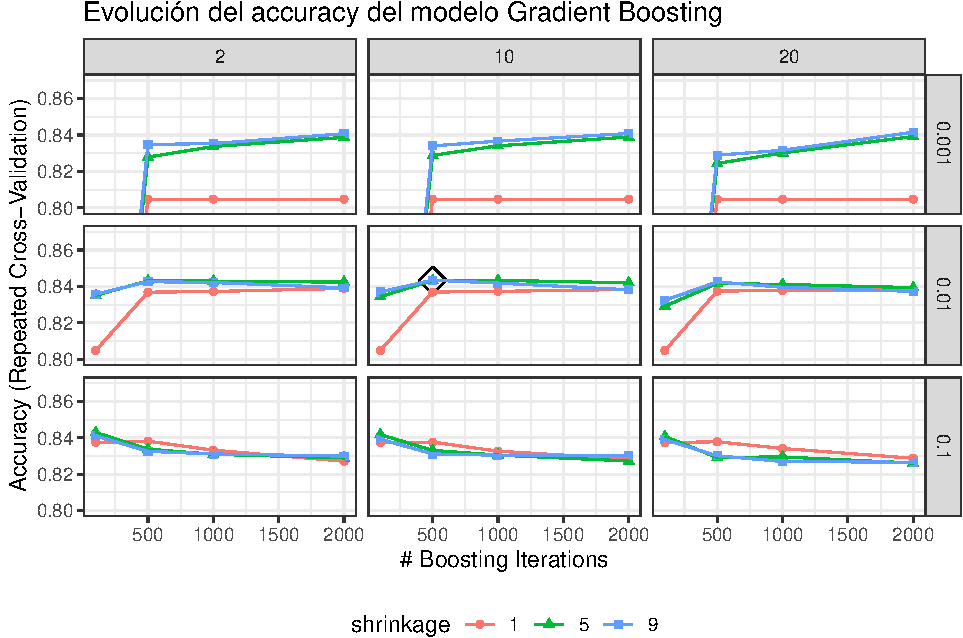
\includegraphics[width=0.9\textwidth]{imagenes/modelos_varios/unnamed-chunk-28-1.pdf}
	%\includegraphics[width=0.25\textwidth]{mesh}
	\caption{Evolución de Accuracy en modelos Gradient Boosting para determinar hiperparámetros}
	\label{fig:rf_hiperparam}
\end{figure}


%-------------------------------------------------%
\subsubsection{Modelar}
%-------------------------------------------------%

En este caso pasa algo similar que con RandomForest. Cuando se usa el conjunto de entrenamiento para generar modelos mediante cross-validation con los hiperparámetros optimizados, se obtiene un Accuracy promedio del 84,34\%. Sin embargo, cuando este mismo métodos y utilizando los mismos hiperparámetros se emplea sin subdivisión de validación (usando todo el conjunto como train), se obtiene un accuracy del 87,4\%. Por lo tanto, está un poco sobreajustado pero no hay tanta diferencia como lo era con RandomForest.





%-------------------------------------------------%
\subsubsection{Describir el modelo}
%-------------------------------------------------%

Se evalúa el modelo con el conjunto de Test. En esta oportunidad se obtiene  Accuracy de 83.83\%. \ref{tab:MatrizConf_boosting} \ref{tab:metricas_boosting}

\begin{table}[!h]
	
	\caption{\label{tab:MatrizConf_boosting}Matriz de Confusión del método: boosting }
	\centering
	\begin{tabular}[t]{lcc}
		\toprule
		\multicolumn{1}{c}{Prediccion} & \multicolumn{1}{c}{Referencia} & \multicolumn{1}{c}{ } \\
		\cmidrule(l{3pt}r{3pt}){1-1} \cmidrule(l{3pt}r{3pt}){2-2}
		\rowcolor{black}  \multicolumn{1}{c}{\textcolor{white}{\textbf{ }}} & \multicolumn{1}{c}{\textcolor{white}{\textbf{0}}} & \multicolumn{1}{c}{\textcolor{white}{\textbf{1}}}\\
		\midrule
		\rowcolor{gray!6}  0 & 678 & 135\\
		1 & 89 & 465\\
		\bottomrule
	\end{tabular}
\end{table}

\begin{table}[!h]
	
	\caption{\label{tab:metricas_boosting}Métricas del método: boosting }
	\centering
	\begin{tabular}[t]{cc}
		\toprule
		\rowcolor{black}  \multicolumn{1}{c}{\textcolor{white}{\textbf{metricas}}} & \multicolumn{1}{c}{\textcolor{white}{\textbf{valor}}}\\
		\midrule
		\rowcolor{gray!6}  Accuracy & 0.8361\\
		Kappa & 0.6645\\
		\rowcolor{gray!6}  AccuracyLower & 0.8154\\
		AccuracyUpper & 0.8553\\
		\rowcolor{gray!6}  AccuracyNull & 0.5610\\
		\addlinespace
		AccuracyPValue & 0.0000\\
		\rowcolor{gray!6}  McnemarPValue & 0.0026\\
		Sensitivity & 0.7750\\
		\rowcolor{gray!6}  Specificity & 0.8839\\
		Pos Pred Value & 0.8393\\
		\addlinespace
		\rowcolor{gray!6}  Neg Pred Value & 0.8339\\
		Precision & 0.8393\\
		\rowcolor{gray!6}  Recall & 0.7750\\
		F1 & 0.8058\\
		\rowcolor{gray!6}  Prevalence & 0.4389\\
		\addlinespace
		Detection Rate & 0.3401\\
		\rowcolor{gray!6}  Detection Prevalence & 0.4052\\
		Balanced Accuracy & 0.8294\\
		\bottomrule
	\end{tabular}
\end{table}



%-------------------------------------------------%
\subsection{Modelo: Support Vector machine (SVM)}
%-------------------------------------------------%

Este algoritmo se basa en la separación de las clases con hiperplanos y
utilizando kernels para aumentar las dimensiones.

%-------------------------------------------------%
\subsubsection{Determinar parámetros del modelo}
%-------------------------------------------------%
Se utiliza el paquete kernlab que tiene 2 hiperparámetros:

\begin{itemize}
	\item
	sigma: coeficiente del kernel radial. Se prueban los valores: 0.001,
	0.01, 0.1, 0.5, 1.
	\item
	C: penalización por violaciones del margen del hiperplano. se prueban
	los valores: 1, 20, 50, 100, 200, 500, 700.
\end{itemize}

Los mejores resultados a través de las iteraciones de los modelos
generados fue con los valores: sigma = 0.001 y C = 100. Los mismos se
contrastan con los valores de Accuracy obtenidos en cada modelo y cuya
evolución puede verse en el grafico \ref{fig:svm_hiperparam}.



\begin{figure}[!htb]
	\centering
	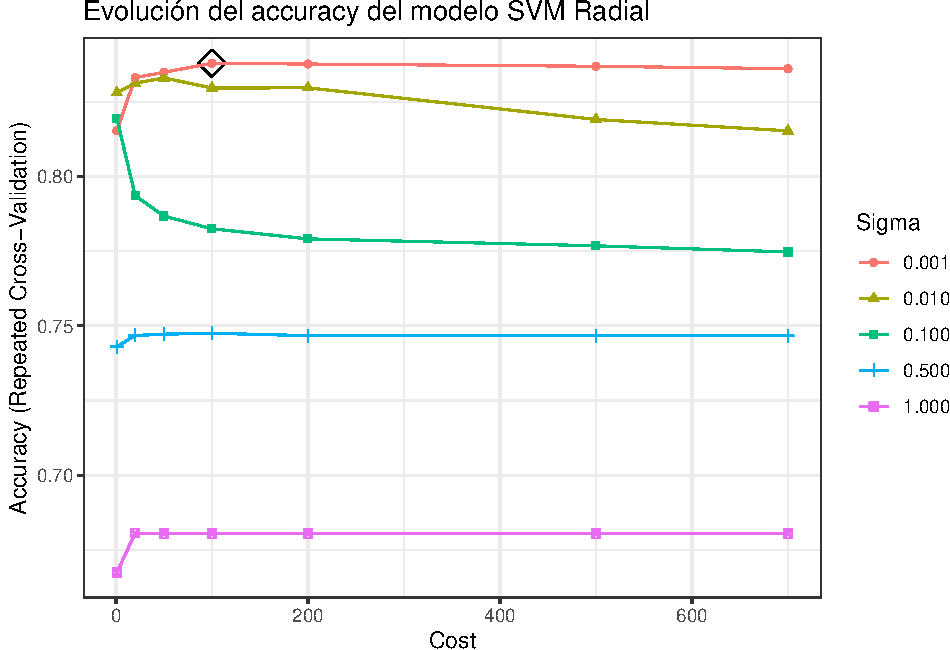
\includegraphics[width=0.78\textwidth]{imagenes/modelos_varios/unnamed-chunk-32-1.pdf}
	%\includegraphics[width=0.25\textwidth]{mesh}
	\caption{Evolución de Accuracy en modelos SVM para determinar hiperparámetros}
	\label{fig:svm_hiperparam}
\end{figure}



%-------------------------------------------------%
\subsubsection{Modelar}
%-------------------------------------------------%

En entrenamiento se consigue un Accuracy de 83.79\% (con validation) y
85.11\% sin validación. Aparenta ser un modelo robusto.


%-------------------------------------------------%
\subsubsection{Describir el modelo}
%-------------------------------------------------%

Evaluando en el conjunto de Test se obtiene 84.2\% de Accuracy. Es el Modelo que mejor resultados da con esta métrica y además es robusto. Para mas información del modelo se detalla la Matriz de Confusión \ref{tab:MatrizConf_SVMradial} y Algunas métricas \ref{tab:metricas_SVMradial}.

\begin{table}[!h]
	
	\caption{\label{tab:metricas_SVMradial}Métricas del metodo: SVMradial }
	\centering
	\begin{tabular}[t]{cc}
		\toprule
		\rowcolor{black}  \multicolumn{1}{c}{\textcolor{white}{\textbf{metricas}}} & \multicolumn{1}{c}{\textcolor{white}{\textbf{valor}}}\\
		\midrule
		\rowcolor{gray!6}  Accuracy & 0.8419\\
		Kappa & 0.6732\\
		\rowcolor{gray!6}  AccuracyLower & 0.8215\\
		AccuracyUpper & 0.8609\\
		\rowcolor{gray!6}  AccuracyNull & 0.5610\\
		\addlinespace
		AccuracyPValue & 0.0000\\
		\rowcolor{gray!6}  McnemarPValue & 0.0000\\
		Sensitivity & 0.7366\\
		\rowcolor{gray!6}  Specificity & 0.9243\\
		Pos Pred Value & 0.8840\\
		\addlinespace
		\rowcolor{gray!6}  Neg Pred Value & 0.8177\\
		Precision & 0.8840\\
		\rowcolor{gray!6}  Recall & 0.7366\\
		F1 & 0.8036\\
		\rowcolor{gray!6}  Prevalence & 0.4389\\
		\addlinespace
		Detection Rate & 0.3233\\
		\rowcolor{gray!6}  Detection Prevalence & 0.3657\\
		Balanced Accuracy & 0.8305\\
		\bottomrule
	\end{tabular}
\end{table}


\begin{table}[!h]
	
	\caption{\label{tab:MatrizConf_SVMradial}Matriz de Confusión del método: SVMradial }
	\centering
	\begin{tabular}[t]{lcc}
		\toprule
		\multicolumn{1}{c}{Prediccion} & \multicolumn{1}{c}{Referencia} & \multicolumn{1}{c}{ } \\
		\cmidrule(l{3pt}r{3pt}){1-1} \cmidrule(l{3pt}r{3pt}){2-2}
		\rowcolor{black}  \multicolumn{1}{c}{\textcolor{white}{\textbf{ }}} & \multicolumn{1}{c}{\textcolor{white}{\textbf{0}}} & \multicolumn{1}{c}{\textcolor{white}{\textbf{1}}}\\
		\midrule
		\rowcolor{gray!6}  0 & 709 & 158\\
		1 & 58 & 442\\
		\bottomrule
	\end{tabular}
\end{table}



\clearpage

%-------------------------------------------------%
\subsection{Modelos: Selección de Variables y Modelos - Alternativa 1}
%-------------------------------------------------%

Los modelos anteriores se han generado con el dataset completo, es decir, utilizando todas las variables disponibles.\\

En este caso, debido al estudio de variables \ref{analisis-var_importantes} y como se mencionó en \ref{conjunto_datos}, se comprobaron mejores resultados
con datasets utilizando únicamente variables seleccionadas. En este caso son 10 variables de las 24 disponibles:\\

``ciclo\_lectivo\_de\_cursada'', ``tipo\_de\_aprobacion\_libre'',
``Turno\_Noche'', ``tipo\_de\_aprobacion\_no\_firmo'', ``Aprobado''
``Turno\_Tarde'', ``Nota\_max\_prom'', ``tipo\_de\_aprobacion\_firmo'',
``Turno\_Manana'' y ``cant\_resursada\_regular''.\\


Por lo que se seleccionaron 2 métodos, para realizar todo el proceso
anterior nuevamente pero solamene teniendo en cuenta estos predictores.\\


Los modelos seleccionados para estas pruebas son: Regresión logística y
RandomForest.


%-------------------------------------------------%
\subsubsection{Determinar parámetros del modelo}
%-------------------------------------------------%

Las grillas de pruebas son, para cada modelo, las mismas utilizadas oportunamente.\\

Se detallan los nuevos parámetros óptimos encontrados: 
RandomForest: mtry = 3, splitrule = gini y min.node.size = 30\\
Regresión Logistica: (sin parametros)

%-------------------------------------------------%
\subsubsection{Modelar}
%-------------------------------------------------%

Los valores de Accuracy obtenidos en entrenamiento:\\
Random Forest: 84,34\% (con validation) y 91,03\% (solo train).\\
Regresión logística: 83,13\% (con validación y 83,45\% (solo train)



%-------------------------------------------------%
\subsubsection{Describir el modelo}
%-------------------------------------------------%

Se evalúan los modelos con el conjunto de Test.
Los Nuevos Valores correspondinetes a la métrica Accuracy en los modelos de regresión logística (Reg\_Logística) y RandomForest (RandomForest) son 83,39\% y 84,05\% respectivamente. %\ref{tab:metricas_RandomForest} \ref{tab:metricas_Reg_logistica}

%-------------------------------------------------%
\subsection{Modelos: Selección de Variables y Modelos - Alternativa 2}
%-------------------------------------------------%

En este caso, se quieren evaluar algunos métodos pero sin tener en cuenta la variable mas importante ``ciclo\_lectivo\_de\_cursada''.\\
Al modificar los datos de entrada, se realiza un nuevo análisis sobre selección de features sin tener en cuenta la variable mencionada. Este análisis determina que para obtener el mejor resultado evaluando la métrica accuracy, deben utilizarse todo el resto de los predictores disponibles. \\

%En este caso, debido al estudio de variables \ref{analisis-var_importantes} y como se mencionó en \ref{conjunto_datos}

Se seleccionaron 5 métodos, para este nuevo análisis: Regresión logística, RandomForest, SVM, C5.0 y GradientBoosting.


%-------------------------------------------------%
\subsubsection{Determinar parámetros del modelo}
%-------------------------------------------------%

Las grillas de pruebas son, para cada modelo, las mismas utilizadas oportunamente.

Se detallan los nuevos parámetros óptimos encontrados: 
RandomForest: mtry = 7, splitrule = gini y min.node.size = 10.
\\
Regresión Logística (sin parametros)\\
GBM: n.trees = 2000, interaction.depth = 2, shrinkage = 0.01
y n.minobsinnode = 15\\
SVM: sigma = 0.001 y C = 200
C5.0: (sin parámetros)


%-------------------------------------------------%
\subsubsection{Modelar}
%-------------------------------------------------%

Se ejecutan los modelos y se obtienen los sigientes valores en la métrica Accuracy:\\
Regresion Logística: 77,31\% (con validación), 77,68\% (con train)\\
RandomForest: 78,28\% (con validación), 96,74\% (con train)\\
GBM: 77,84\% (con validación), 79,63\% (con train)\\
C5.0: 75,36\% (con validación), 81,47\% (con train)\\
SVM: 78,1\% (con validación), 79,88\% (con train)

%-------------------------------------------------%
\subsubsection{Describir el modelo}
%-------------------------------------------------%

Se predicen las observaciones del conjunto de Test y contrastando con el target, se obtienen los siguientes valores en la métrica Accuracy:\\
GradientBoosting: 75,2\%,\\
C5.0: 75,34\%,\\
Regresión Logística: 77,17\%\\
SVM: 78,20\%\\
RandomForest: 78,49\%


%%-------------------------------------------------%
%\subsection{Modelo: xxx}
%%-------------------------------------------------%
%\todorevisar{poner definicion de modelo corta aca o en la seccion que esta mas arriba}
%
%
%%-------------------------------------------------%
%\subsubsection{Determinar parámetros del modelo}
%%-------------------------------------------------%
%
%%-------------------------------------------------%
%\subsubsection{Modelar}
%%-------------------------------------------------%
%
%%-------------------------------------------------%
%\subsubsection{Describir el modelo}
%%-------------------------------------------------%
